% Python for Scientists: Lesson 2
% Author: Marshall Ward
%=============================================================================%
\documentclass[red]{beamer}

% Font configuration
\usepackage{pxfonts}
%\usepackage{eulervm}
%\usepackage{type1cm}
%\usepackage{fourier}

% Packages
\usepackage{listings}

\usepackage{color}
\definecolor{ltblue}{rgb}{0.9, 0.9, 1.0}
\definecolor{dkgreen}{rgb}{0,0.6,0}
\definecolor{gray}{rgb}{0.5,0.5,0.5}
\definecolor{mauve}{rgb}{0.58,0,0.82}

\usepackage{hyperref}

% Directory Structure
\graphicspath{{figures/}}

% Beamer configuration
\usetheme{Frankfurt}
%-----------------------------------------------------------------------------%
\AtBeginSection[]
{
   \begin{frame}
        \frametitle{Outline}
        \tableofcontents[currentsection]
    \end{frame}
}
%-----------------------------------------------------------------------------%
\title{Python for Scientists: NumPy}
%=============================================================================%
\begin{document}
% Listings settings
\lstset{
    language=Python,
    basicstyle=\ttfamily,
    showspaces=false,
    showstringspaces=false,
    backgroundcolor=\color{ltblue},
    numberstyle=\tiny\color{gray},        % line number style
    keywordstyle=\color{blue},          % keyword style
    commentstyle=\color{dkgreen},       % comment style
    stringstyle=\color{mauve}         % string literal style
}
%-----------------------------------------------------------------------------%
\begin{frame}
    \titlepage
\end{frame}
%=============================================================================%
\section[Intro]{What is NumPy?}
%-----------------------------------------------------------------------------%
\frame{
    \frametitle{What is NumPy?}
    
    NumPy is a Python interface between two things:
    \begin{itemize}
        \item A numerical array (vector) in memory
        \item A set of numerical C libraries\\
              (usually based on ATLAS or MKL)
    \end{itemize}
    
    When you use NumPy, you are really using a Python interface to pre-compiled C code.
}
%-----------------------------------------------------------------------------%
\frame{
    \frametitle{NumPy vs. Matlab vs. Bytecode}

    Comparison of $\nabla^2 u = 0$ solvers ($500\times500$, 100 iterations):
    
    \begin{columns}
        \column{0.4\textwidth}
        \begin{table}
            \begin{tabular}{|c|c|}
                \hline
                Platform & Time (s) \\
                \hline \hline
                Python & $\sim$1500.0 \\
                \hline
                NumPy & 29.3 \\
                \hline
                Matlab & $\sim$29.0 \\
                \hline
                Octave & $\sim$60.0 \\
                \hline
                Blitz (C++) & 9.5 \\
                \hline
                Fortran & 2.5 \\
                \hline
                C & 2.2 \\
                \hline
            \end{tabular}
        \end{table}
        \column{0.6\textwidth}
        \begin{center}
            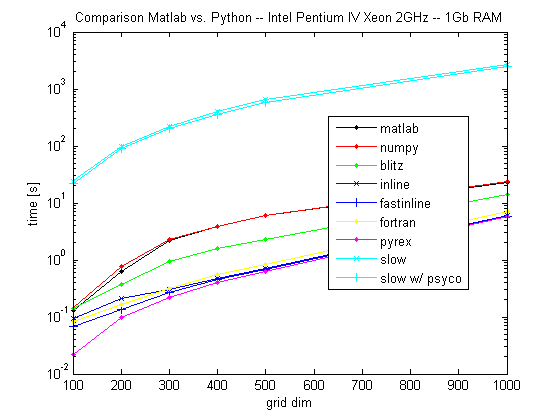
\includegraphics[width=\textwidth]{numpy_perf1.png}
        \end{center}
    \end{columns}

    (Probably using MKL)

    {\tiny \href{http://www.scipy.org/PerformancePython}{http://www.scipy.org/PerformancePython}}\\
    {\tiny \href{http://lbolla.info/blog/2007/04/11/numerical-computing-matlab-vs-pythonnumpyweave/}{http://lbolla.info/blog/2007/04/11/numerical-computing-matlab-vs-pythonnumpyweave/}}
}
%=============================================================================%
\section[Arrays]{NumPy Arrays}
%-----------------------------------------------------------------------------%
\begin{frame}[fragile]
    \frametitle{NumPy Array Generation}

    Convert a list to a NumPy array:
    \begin{lstlisting}
>>> import numpy as np
>>> list = [1, 2, 3, 4, 5]
>>> x = np.array(list)
>>> x
array([1, 2, 3, 4, 5])
>>> x.dtype
dtype('int64')
    \end{lstlisting}
    NumPy arrays have values and a data type (\textit{dtype}).
\end{frame}
%-----------------------------------------------------------------------------%
\begin{frame}[fragile]
    \frametitle{NumPy Array Generation}

    \lstinline|arange()| is similar to \lstinline|range()| for lists:
    \begin{lstlisting}
>>> np.arange(5)
array([0, 1, 2, 3, 4])
>>> np.arange(5.)
array([0., 1., 2., 3., 4.])
    \end{lstlisting}
    
    \lstinline|zeros| for pre-allocation:
    \begin{lstlisting}
>>> np.zeros([2, 3])    # Input is a list
array([[ 0., 0., 0.],
       [ 0., 0., 0.]])
    \end{lstlisting}
\end{frame}
%-----------------------------------------------------------------------------%
\begin{frame}[fragile]
    \frametitle{NumPy Grid Generation}
   
    Suppose you want to construct a numerical grid.\\
    e.g. $x = x_0 + j \Delta x$, \ $\Delta x = (x_1 - x_0) / N$
    \\~\\
    \lstinline|arange()| uses $\Delta x$ and excludes $x_1$:
    \begin{lstlisting}
>>> x = np.arange(3., 6., 0.5)
array([ 3. ,  3.5,  4. ,  4.5,  5. ,  5.5])
    \end{lstlisting}
    \lstinline|linspace()| uses $N+1$ and includes $x_1$:
    \begin{lstlisting}
>>> x = np.linspace(0., 1., 6)
array([ 0. ,  0.2,  0.4,  0.6,  0.8,  1. ])
    \end{lstlisting}
\end{frame}
%-----------------------------------------------------------------------------%
\begin{frame}[fragile]
    \frametitle{NumPy Arithmetic}
    
    All NumPy operations are vectorized:
    \begin{lstlisting}
>>> x = np.linspace(0., 4., 5)
>>> y = np.linspace(-2., -2., 5)
>>> 2*x
array([ 0.,  2.,  4.,  6.,  8.])
>>> x+y
array([-2.,  0.,  2.,  4.,  6.])
    \end{lstlisting}

    Most mathematical functions are supported:
    \begin{lstlisting}
>>> np.exp(x)
>>> np.arctan(x)
>>> np.pi
    \end{lstlisting}
\end{frame}
%-----------------------------------------------------------------------------%
\begin{frame}[fragile]
    \frametitle{Inefficient Arithmetic}

    Never do this:
    \begin{lstlisting}
>>> for i in range(10):
        z[i] = x[i] + y[i]
    \end{lstlisting}
    It will send 10 separate jobs to the C libraries.
    \\~\\
    Always try to do vectorized calculations:
    \begin{lstlisting}
>>> z = x+y
    \end{lstlisting}
    It only sends one job.
\end{frame}
%-----------------------------------------------------------------------------%
\frame{
    \frametitle{Arithmetic Quiz}

    Use \lstinline|np.mean()| to estimate the mean value of $f(x)$ over $[-1,1]$:

    \begin{columns}
        \column{0.5\textwidth}        
            \[ \frac{1}{2} \int_{-1}^{1} f(x) \; dx \]
        \column{0.5\textwidth}    
            \begin{itemize}
                \item $f(x) = \sin x$
                \item $f(x) = 1/(1 + x^2)$
                \item $f(x) = x^2 \exp(-x^2)$
            \end{itemize}
    \end{columns}

    \onslide<2->{\lstinputlisting{scripts/np_mean.py}}
}
%=============================================================================%
\section[Dimensions]{Multidimensional Arrays}
%-----------------------------------------------------------------------------%
\begin{frame}[fragile]
    \frametitle{Multidimensional Arrays}

    NumPy supports multidimensional arrays:
    \begin{lstlisting}
>>> x = np.zeros((3,4))
>>> x
array([[ 0.,  0.,  0.,  0.],
       [ 0.,  0.,  0.,  0.],
       [ 0.,  0.,  0.,  0.]])
>>> x[:,0]
array([ 0.,  0.,  0.,  0.])
>>> x[0] # or x[0,:]
array([ 0.,  0.,  0.])
    \end{lstlisting}
    NumPy arrays support comma-separated dimension indexing

\end{frame}
%-----------------------------------------------------------------------------%
\begin{frame}[fragile]
    \frametitle{Grid Arrays}

    \lstinline|np.meshgrid()| lets you generate 2D grids from 1D axes:
    \begin{lstlisting}
>>> x_axis = np.linspace(-1., 1., 11)
>>> y_axis = np.linspace(0., 1., 6)
>>> x, y = np.meshgrid(x, y)
    \end{lstlisting}
    Inspect the shape of \lstinline|x| and \lstinline|y|. How are dimensions arranged?

\end{frame}
%-----------------------------------------------------------------------------%
\begin{frame}
    \frametitle{Multidimensional Quiz}

    Construct $f(x,y) = \sin x \cosh y$ on $(x,y) = [-1,1]\times[0,1]$.
    \\~\\
    How would you compute $df/dx$ and $df/dy$?
    \onslide<2->{
        \lstinputlisting{scripts/2d_grid.py}
    }
\end{frame}
%-----------------------------------------------------------------------------%
\begin{frame}[fragile]
    \frametitle{Reshaping}
    Two ways to reshape an array:
    \\~\\
    \lstinline|reshape()| outputs a new reshaped array:
    \begin{lstlisting}
>>> x = np.arange(12)
>>> x.reshape(3,4)
    \end{lstlisting}
    
    \lstinline|resize()| (or \lstinline|x.shape|) changes a shape:
    \begin{lstlisting}
>>> x.resize(6,2)
>>> x
>>> x.shape = 2,6
>>> x
    \end{lstlisting}
\end{frame}
%-----------------------------------------------------------------------------%
\begin{frame}[fragile]
    \frametitle{Broadcasting}

    Arithmetic usually requires arrays to be the same shape:
    \begin{lstlisting}
>>> x = np.arange(12).reshape(3,4)
>>> y = np.arange(12).reshape(4,3)
>>> x*y   # Does this work?
    \end{lstlisting}

    But \textit{broadcasting} will copy outer dimensions inward:
    \begin{lstlisting}
>>> x = np.ones(12).reshape(3,4)
>>> y = np.arange(4)
>>> x*y     # Outer dimension matches
    \end{lstlisting}
    As long as the last dimensions match, you can broadcast.
\end{frame}
%-----------------------------------------------------------------------------%
\begin{frame}[fragile]
    \frametitle{Extending Array Dimensions}

    What if you need to multiply along the first dimension?
    \begin{lstlisting}
>>> x = np.ones((3,4))
>>> y = np.arange(3)
>>> x * y                   # Won't work
>>> x * y[:, np.newaxis]    # Works!
    \end{lstlisting}
    \lstinline|np.newaxis| extends any missing dimension!
    \\~\\
    (Also see \lstinline|np.tile| and \lstinline|np.repeat|)
\end{frame}
%-----------------------------------------------------------------------------%
\begin{frame}[fragile]
    \frametitle{Combining Arrays}

    Combine two arrays along some dimension:
    \begin{lstlisting}
>>> x = np.arange(5)
>>> y = np.arange(5)
>>> np.hstack((x,y))    # Stack on axis=0
>>> np.vstack((x,y))    # Stack on axis=1
    \end{lstlisting}

    Use \lstinline|np.concatenate| for higher dimensions:
    \begin{lstlisting}
>>> x = np.ones((4,3,2))
>>> y = np.ones((4,3,1))
>>> np.concatenate((x,y),axis=2)
    \end{lstlisting}
\end{frame}
%=============================================================================%
\section[Copying]{Copying NumPy Arrays}
%-----------------------------------------------------------------------------%
\begin{frame}[fragile]
    \frametitle{NumPy Variables are References}

    NumPy arrays are mutable, so NumPy variables are \textit{references}.
    \\~\\
    Try these commands, then look at \lstinline|x| and \lstinline|y|:
    \begin{lstlisting}
>>> x = np.arange(5)
>>> y = x
>>> x[0] = 5
    \end{lstlisting}
    Changing x will change y
\end{frame}
%-----------------------------------------------------------------------------%
\begin{frame}[fragile]
    \frametitle{Copying NumPy Arrays}

    \textit{Deep Copy}: Duplicate the array in memory
    \begin{lstlisting}
>>> x = np.arange(10)
>>> y = np.copy(x)
>>> x[0] = 5
>>> x
>>> y
    \end{lstlisting}
\end{frame}
%-----------------------------------------------------------------------------%
\begin{frame}[fragile]
    \frametitle{NumPy Views}

    \textit{View}: Same Data, different properties\\
    (i.e. a ``different view'' of the data)
    \\~\\
    Try these commands, then look at \lstinline|x| and \lstinline|y|:
    \begin{lstlisting}
>>> x = np.arange(12)
>>> y = x[:]    # y = x.view() also works
>>> y.shape = 3, 4
>>> x[0] = 12
    \end{lstlisting}
    Note: \lstinline|y = x[:]| copies lists, but creates NumPy \textit{views}!
    \\~\\
    Subarrays are also views:
    \begin{lstlisting}
>>> x = np.arange(5)
>>> y = x[:3]
>>> x[0]
    \end{lstlisting}
\end{frame}
%=============================================================================%
\section[I/O]{I/O (Using SciPy)}
%-----------------------------------------------------------------------------%
\begin{frame}[fragile]
    \frametitle{I/O with SciPy}
    
    NumPy has a unique binary data format:
    \begin{lstlisting}
>>> np.save('mydata.npy', data)
>>> data = np.load('mydata.npy')
    \end{lstlisting}

    Several I/O routines are provided by SciPy (scientific python).

    Matlab:
    \begin{lstlisting}
>>> import scipy.io as sio
>>> data = sio.loadmat('mydata.mat')
>>> sio.savemat('mydata.mat', {'var': data})
    \end{lstlisting}
\end{frame}
%-----------------------------------------------------------------------------%
\begin{frame}[fragile]
    \frametitle{SciPy NetCDF Support}

    SciPy provides some NetCDF support (PuPyNeRe):
    \begin{lstlisting}
>>> import scipy.io as sio
>>> x = np.arange(5)
>>> f = sio.netcdf.netcdf_file('out.nc','w')
>>> f.createDimension('xd',5)
>>> x_var = f.createVariable('x','d',('xd',))
>>> x_var[:] = x
>>> f.close()
    \end{lstlisting}
    Also see: \lstinline|netcdf4-python|
\end{frame}
%=============================================================================%
\section{Masked Arrays}
%-----------------------------------------------------------------------------%
\begin{frame}[fragile]
    \frametitle{Masking}

    Filtering with logical operators:
    \begin{lstlisting}
>>> x = np.random.rand(3,4)
>>> x > 0.5
>>> x[(x>0.5)]
    \end{lstlisting}
    This can be useful, but you lose the shape!
\end{frame}
%-----------------------------------------------------------------------------%
\begin{frame}[fragile]
    \frametitle{Masked Arrays}

    NumPy provides Masked Array support: \lstinline|np.ma|:
    \begin{lstlisting}
>>> x = np.random.rand(3,4)
>>> x_m = np.ma.masked_array(x, x>0.5)
>>> print x_m
    \end{lstlisting}
    Support isn't universal, but it's not bad
\end{frame}
%=============================================================================%
\section{Linear Algebra}
%-----------------------------------------------------------------------------%
%=============================================================================%
\section{SciPy}
%-----------------------------------------------------------------------------%
\frame{
    \frametitle{SciPy}

    SciPy provides lots of useful science tools:
    \begin{itemize}
        \item \lstinline|scipy.interpolate|\\
            Grid interpolation tools
        \item \lstinline|scipy.stats|, \lstinline|scipy.random|\\
            Statistical analysis
        \item \lstinline|scipy.signal|\\
            Filtering, Signal Processing
    \end{itemize}
    and many more
}
%=============================================================================%
\end{document}
